\item \begin{enumerate}
        \item Sea $R_\alpha:\R^2\to\R^2$ la función que define la rotación en un ángulo $\alpha$ (fijo) en sentido antihorario, es decir \[R_\alpha(x,y)=(x \cos(\alpha)-y\sin(\alpha),x\sin(\alpha)+y\cos(\alpha))\quad\forall(x,y)\in\R^2\]
            \begin{enumerate}
                \item[1)] Probar que $R_\alpha$ es una transformación lineal para cualquier valor del ángulo $\alpha$ fijo.
                    \begin{mdframed}[style=s]
                        Sean $u,v\in\R^2,\lambda\in\R, u=(u_1,u_2),v=(v_1,v_2)$
                        \begin{align*}
                            T(u+v)&=T((u_1,u_2)+(v_1,v_2))\\
                            \text{Suma en }\R^2&=T(u_1+v_1,u_2+v_2)\\
                            \text{Definición T}&=((u_1+v_1)\cos(\alpha)-(u_2+v_2)\sin(\alpha),(u_1+v_1)\sin(\alpha)+(u_2+v_2)\cos(\alpha))\\
                            \text{Distributividad}&=(u_1\cos(\alpha)-u_2\sin(\alpha)+v_1\cos(\alpha)-v_2\sin(\alpha),\\
                            &\qquad u_1\sin(\alpha)+u_2\cos(\alpha)+v_1\sin(\alpha)+v_2\cos(\alpha))\\
                            \text{Suma en }\R^2&=(u_1\cos(\alpha)-u_2\sin(\alpha),u_1\sin(\alpha)+u_2\cos(\alpha))\\
                            &\qquad +(v_1\cos(\alpha)-v_2\sin(\alpha),v_1\sin(\alpha)+v_2\cos(\alpha))\\
                            \text{Definición T}&=T(u_1,u_2)+T(v_1,v_2)\\
                            &=T(u)+T(v)
                        \end{align*}
                        Por otra parte, sea $v=(v_1,v_2)\in\R^2,\lambda\in\R$
                        \begin{align*}
                            T(\lambda v)&=T(\lambda(v_1,v_2))\\
                            \text{Producto por escalar }\R^2&=T(\lambda v_1,\lambda v_2)\\
                            \text{Definición T}&=((\lambda v_1)\cos(\alpha)-(\lambda v_12)\sin(\alpha),(\lambda v_1)\sin(\alpha)+(\lambda v_2)\cos(\alpha))\\
                            \text{Factor común}&=\lambda(v_1\cos(\alpha)-v_2\sin(\alpha),v_1\sin(\alpha)+v_2\cos(\alpha))\\
                            \text{Definición T}&=\lambda T(v_1,v_2)\\
                            &=\lambda T(v)
                        \end{align*}
                        Por lo tanto, $T$ es una transformación lineal.
                    \end{mdframed}
                \item[2)] Determinar la imagen por $R_{\frac{\pi}{2}}$ de $P=(0,3),Q(3,1)$ y $S=(1,-1)$. Graficar el triángulo $PQS$ y su transformado en el mismo sistema de coordenadas.
                    \begin{mdframed}[style=s]
                        \[R_{\frac{\pi}{2}}(0,3)=(-3,0)\qquad R_{\frac{\pi}{2}}(3,1)=(-1,3)\qquad R_{\frac{\pi}{2}}(1,-1)=(1,1)\]
                        En la Figura 4 se puede ver como queda el triángulo transformado
                        \begin{center}
                            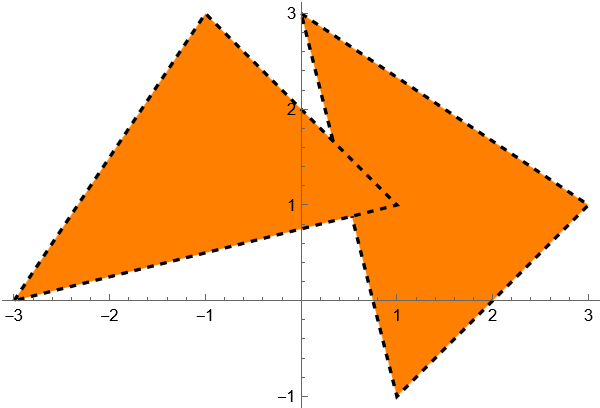
\includegraphics[width=0.4\textwidth]{img/ej11a.png}\\
                            Figura 4. Triángulo antes y después de ser transformado por $R_{\frac{\pi}{2}}$
                        \end{center}
                    \end{mdframed}
            \end{enumerate}
        \item Sea $S_Y:\R^2\to\R^2$ la función simetría respecto al eje $y$, es decir\[S_Y(x,y)=(-x,y)\quad\forall(x,y)\in\R^2.\]
            \begin{enumerate}
                \item[1)] Probar que $S_Y$ es una transformación lineal.\pagebreak
                    \begin{mdframed}[style=s]
                        Sean $u=(u_x,u_y),v=(v_x,v_y)\in\R^2,\alpha\in\R$
                        \begin{align*}
                            S_Y(\alpha u+v)&=S_Y(\alpha(u_x,u_y)+(v_x,v_y))\\
                            \text{Suma y prod por escalar}&=S_Y(\alpha u_x+v_x,\alpha u_y+v_y)\\
                            \text{Definición }S_Y&=(-(\alpha u_x+v_x),\alpha u_y+v_y)\\
                            \text{Suma en }\R^2&=(-\alpha u_x,\alpha u_y)+(-v_x,v_y)\\
                            \text{Prod por escalar}&=\alpha(-u_x,u_y)+(-v_x,v_y)\\
                            \text{Definición }S_Y&=\alpha S_Y(u_x,u_y)+S_Y(v_x,v_y)\\
                            &=\alpha S_Y(u)+S_Y(v)
                        \end{align*}
                    \end{mdframed}
                \item Determinar la imagen por $S_Y$ de $A=(0,1),B=(2,4),C=(4,3)$ y $D=(2,0)$. Graficar el rectángulo $ABCD$ y su transformado en el mismo sistema de coordenadas.
                    \begin{mdframed}[style=s]
                        \[S_Y(A)=(0,1)\qquad S_Y(B)=(-2,4)\qquad S_Y(C)=(-4,3)\qquad S_Y(D)=(-2,0)\qquad\]
                        En la Figura 5 se puede ver como queda el rectángulo transformado
                        \begin{center}
                            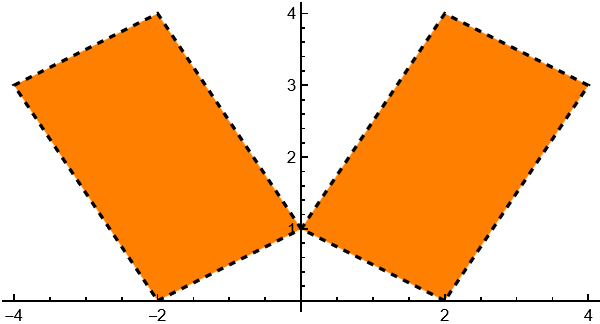
\includegraphics[width=0.4\textwidth]{img/ej11b.png}\\
                            Figura 5. Rectángulo antes y después de ser transformado por $S_Y$
                        \end{center}
                    \end{mdframed}
            \end{enumerate}
        \item Sea $H_k:\R^2\to\R^2$ la función homotecia de razón $k\in\R$ (fijo), es decir\[H_k(x,y)=(kx,ky)\quad\forall(x,y)\in\R^2.\]
            \begin{enumerate}
                \item[1)] Probar que $H_k$ es una transformación lineal para cualquier valor de $k\in\R$ fijo.
                    \begin{mdframed}[style=s]
                        Sean $u=(u_x,u_y),v=(v_x,v_y)\in\R^2,\alpha\in\R$
                        \begin{align*}
                            H_k(\alpha u+v)&=H_k(\alpha(u_x,u_y)+(v_x,v_y))\\
                            \text{Suma y prod por escalar}&=H_k(\alpha u_x+v_x,\alpha u_y+v_y)\\
                            \text{Definición }H_k&=(k(\alpha u_x+v_x),k(\alpha u_y+v_y))\\
                            \text{Suma en }\R^2&=(k\alpha u_x,k\alpha u_y)+(kv_x,kv_y)\\
                            \text{Prod por escalar}&=\alpha(ku_x,ku_y)+(kv_x,kv_y)\\
                            \text{Definición }H_k&=\alpha H_k(u_x,u_y)+H_k(v_x,v_y)\\
                            &=\alpha H_k(u)+H_k(v)
                        \end{align*}
                        Por lo tanto $H_k$ es una transformación lineal.
                    \end{mdframed}
                \item[2)] Determinar la imagen de $H_2$ de $A=(0,-1),B=(1,2)$ y $C=(3,1)$. Graficar el triángulo $ABC$ y su transformado en el mismo sistema de coordenadas.
                    \begin{mdframed}[style=s]
                        \[H_2(0,-1)=(0,-2)\qquad H_2(1,2)=(2,4)\qquad H_2(3,1)=(6,2)\]
                        En la Figura 6 se puede ver como queda el triángulo transformado
                        \begin{center}
                            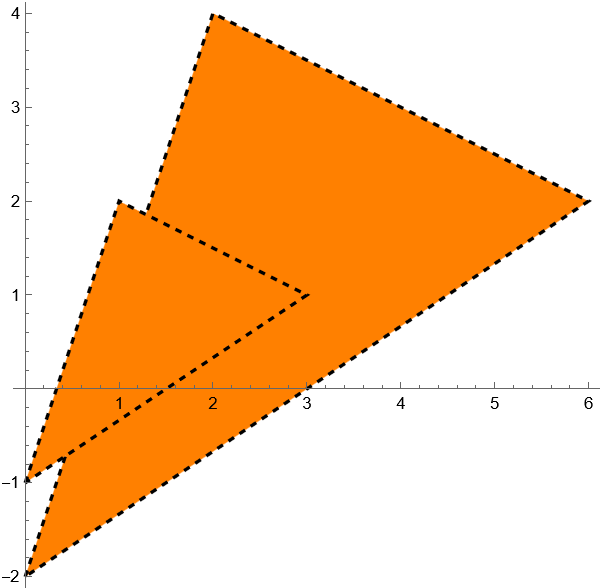
\includegraphics[width=0.4\textwidth]{img/ej11c.png}\\
                            Figura 6. Triángulo antes y después de ser transformado por $H_2$
                        \end{center}
                    \end{mdframed}
            \end{enumerate}
        \item Sea $P_X:\R^2\to\R^2$ la función proyección sobre el eje $x$.
            \begin{enumerate}
                \item[1)] Hallar una expresión analítica para $P_X$ y probar que es una transformación lineal.
                    \begin{mdframed}[style=s]
                        \[P_X(x,y)=(x,0)\]
                        Sean $u=(u_x,u_y),v=(v_x,v_y)\in\R^2,\alpha\in\R$
                        \begin{align*}
                            P_X(\alpha u+v)&=P_X(\alpha(u_x,u_y)+(v_x,v_y))\\
                            \text{Suma y prod por escalar}&=P_X(\alpha u_x+v_x,\alpha u_y+v_y)\\
                            \text{Definición }P_X&=(\alpha u_x+v_x,0)\\
                            \text{Suma en }\R^2&=(\alpha u_x,0)+(v_x,0)\\
                            \text{Prod por escalar}&=\alpha(u_x,0)+(kv_x,0)\\
                            \text{Definición }P_X&=\alpha P_X(u_x,u_y)+P_X(v_x,v_y)\\
                            &=\alpha P_X(u)+P_X(v)
                        \end{align*}
                        Por lo tanto, $P_X$ es una transformación lineal.
                    \end{mdframed}
                \item[2)] Determinar la imagen por $P_X$ de $A=(0,1),B=(2,4),C=(4,3)$ y $D=(2,0)$. Graficar el rectángulo $ABCD$ y su transformado, en el mismo sistema de coordenadas.
                    \begin{mdframed}[style=s]
                        \[P_X(0,1)=(0,0)\qquad P_X(2,4)=(2,0)\qquad P_X(4,3)=(4,0)\qquad P_X(2,0)=(2,0)\qquad \]
                        En la Figura 7 se puede ver como queda el rectángulo transformado
                        \begin{center}
                            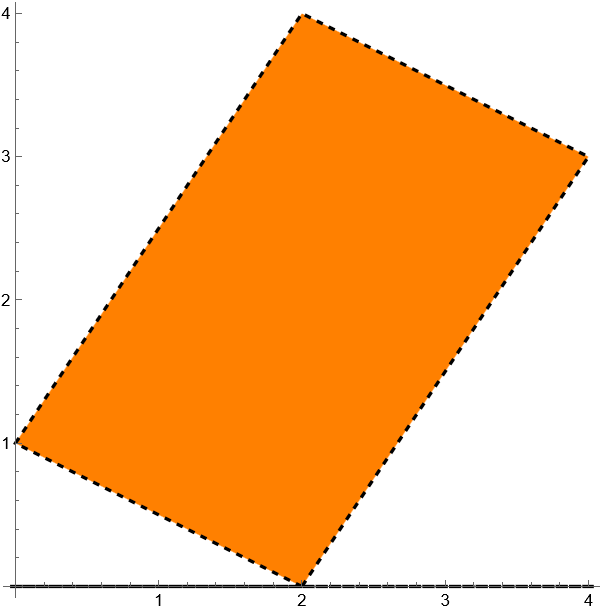
\includegraphics[width=0.4\textwidth]{img/ej11d.png}\\
                            Figura 7. Rectángulo antes y después de ser transformado por $P_X$
                        \end{center}
                    \end{mdframed}
            \end{enumerate}
    \end{enumerate}